\documentclass[a4paper, 12pt]{article}
\usepackage[a4paper,top=1.5cm, bottom=1.5cm, left=1cm, right=1cm]{geometry}
\usepackage{cmap}					% поиск в PDF
\usepackage{mathtext} 				% русские буквы в фомулах
\usepackage[T2A]{fontenc}			% кодировка
\usepackage[utf8]{inputenc}			% кодировка исходного текста
\usepackage[english,russian]{babel}	% локализация и переносы

\usepackage{amsmath}
\usepackage{indentfirst}
\usepackage{longtable}
\usepackage{graphicx}
\usepackage{array}

\usepackage{wrapfig}
\usepackage{siunitx} % Required for alignment
\usepackage{subfigure}
\usepackage{multirow}
\usepackage{rotating}
\usepackage{caption}

\graphicspath{{img/}}


\title{\begin{center}Лабораторная работа №2.2.6\end{center}
Определение энерги активации по температурной зависимости вязкости жидкости}
\author{Рожков А. В. \\ Преподаватель Яворский В. А.}
\date{\today}

\begin{document}
    \pagenumbering{gobble}
    \maketitle
    \newpage
    \pagenumbering{arabic}

    \textbf{Цель работы:} 1) измеренеи объёмов форвакуумной и высоковакуумной частей установки; 2) определение скорости откачки системы в стационарном режиме, а также по ухудшению и по улучшению вакуума.

    \textbf{В работе используются:} вакуумная установка с манометрами: масляным, термопарным и ионизационным.

    \section{Экспериментальная установка}

    \begin{figure}[h]
        \center{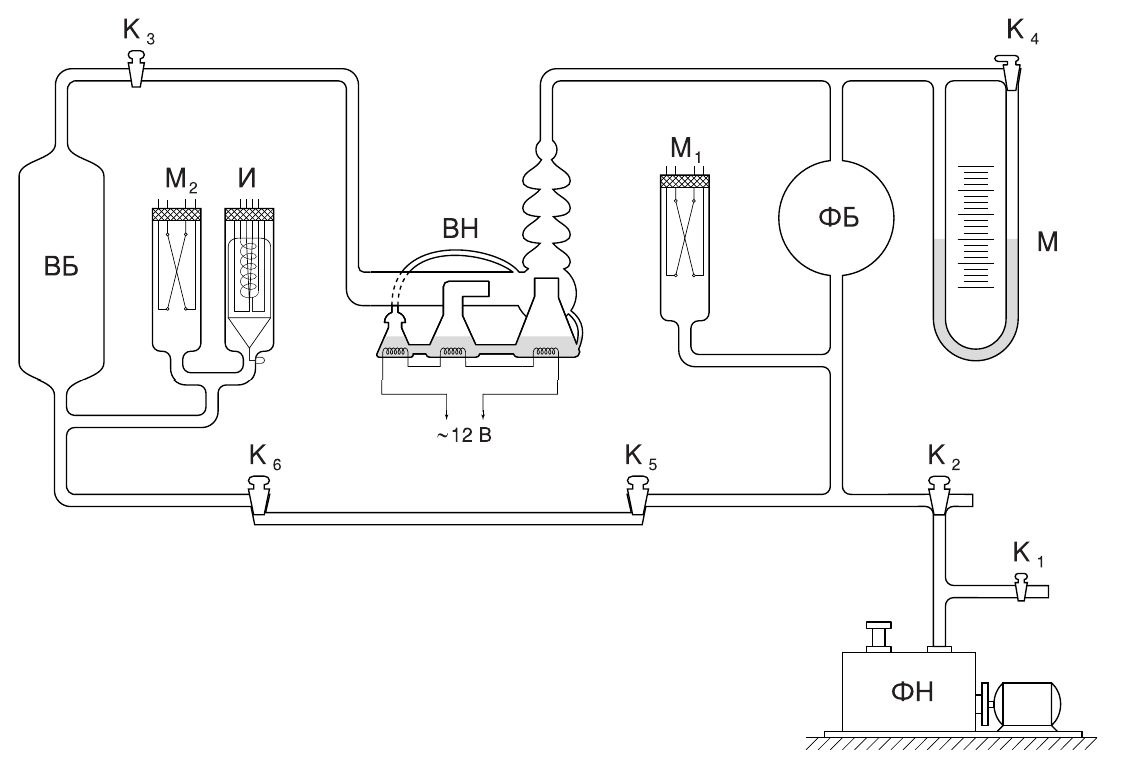
\includegraphics[width=0.8\textwidth]{ustanovka}}
        \caption{Схема экспериментальной установки.}
        \label{ris:ustanovka}
    \end{figure}

    \paragraph{}
    Установка изготовлена из стекла и состоит из форвакуумного баллона (ФБ), высоковакуумного диффузионного насоса (ВН), высоковакуумного баллона (ВБ), масляного (М) и ионизационного (И) манометров, термопарных манометров ($М_1$ и $М_2$), форвакуумного насоса (ФН) и соединительных кранов (Рис. \ref{ris:ustanovka}). Кроме того, в состав установки входят: вариатор (автотрансформатор с регулируемым выходным напряжением), или реостат и амперметр для регулирования тока нагревателя диффузионного насоса.

    \paragraph{Маслянный манометр:}
    Представляет собой U-образную трубку, до половины наполненную вязким маслом, обладающим весьма низким давлением насыщенных паров. Так как плотность масла мала, $\rho = 0,885 г/см^3$ , то при помощи манометра можно измерить только небольшие разности давлений (до нескольких торр). Во время откачки и заполнения установки атмосферным воздухом кран $К_4$ соединяющий оба колена манометра, должен быть открыт во избежание выброса масла и загрязнения установки. Кран $К_4$ закрывается только при измерении давления U-образным манометром.


    \newpage

    \paragraph{Термопарный манометр:}
    Чувствительным элементом манометра является термопара, заключенная в стеклянный баллон. Устройство термопары поясненона (Рис. \ref{ris:termoparni_monometr}). По нити накала НН пропускается ток постоянной величины. Термопара ТТ присоединяется к милливольтметру, показания которого определяются температурой нити накала и зависят от отдачи тепла вокружающее пространство. Потери тепла определяются теплопроводностью нити и термопары, теплопроводностью газа, переносом тепла конвективными потоками газа внутри лампы и теплоизлучением нити (инфракрасноетепловое излучение). В обычном режимелампы основную роль играет теплопроводность газа. При давлениях >1 торр теплопроводность газа, а вместе с ней и ЭДС термопары практически не зависят от давления газа, и прибор не работает. При улучшении вакуума средний свободный пробег молекул становится сравнимым с диаметром нити, теплоотвод падает и температура спая возрастает. При вакууме $~10^{-3}$ торр теплоотвод, осуществляемый газом, становится сравнимым с другими видами потерь теплаи температура нити становится практически постоянной. Градуировочная кривая термопарного манометра приведена на (Рис. \ref{ris:termopara_graduirovka}).

    \begin{figure}[h]
    \centering
    \begin{minipage}{0.3\textwidth}
        \centering
        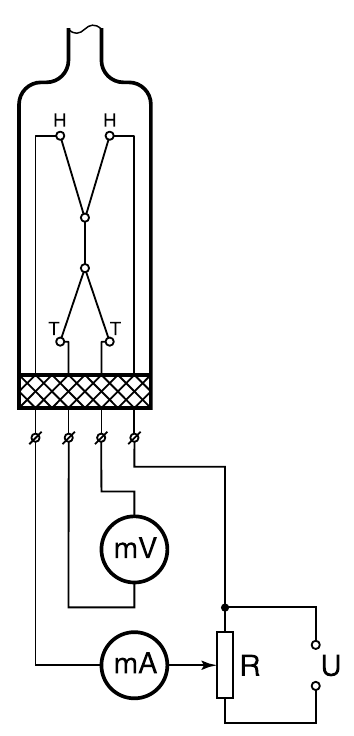
\includegraphics[width=0.9\textwidth]{termoparni_monometr}
        \caption{Схема термопаного манометра.}
        \label{ris:termoparni_monometr}
    \end{minipage}\hfill
    \begin{minipage}{0.7\textwidth}
        \centering
        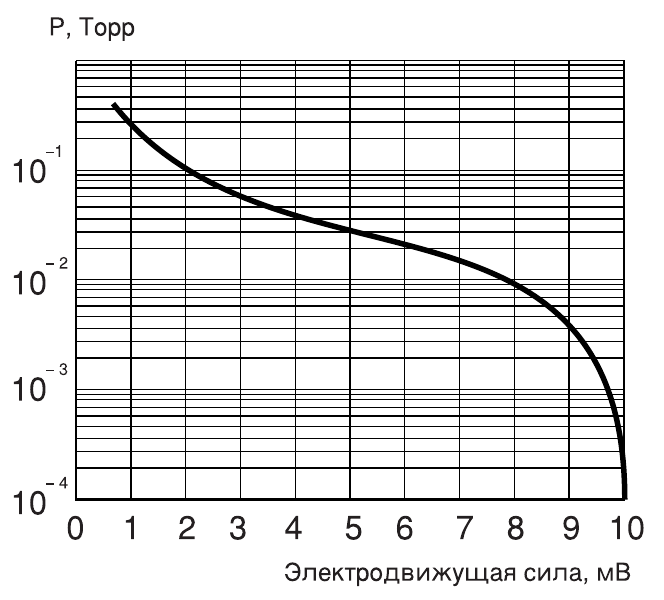
\includegraphics[width=0.9\textwidth]{termopara_graduirovka}
        \caption{Градуировочная кривая термопарного манометра.}
        \label{ris:termopara_graduirovka}
    \end{minipage}
    \end{figure}

    \newpage

    \paragraph{Ионизационный манометр:}
    Схема ионизационного манометра изображена на (Рис. \ref{ris:ionizacionni_monometr}). Он представляет собой трехэлектродную лампу. Электроны испускаются накаленным катодом и увлекаются электрическим полем к аноду, имеющему вид спирали. Проскакивая за ее витки,электроны замедляются полем коллектора и возвращаются к катоду, а от него вновь увлекаются к аноду. Прежде чем осесть на аноде, они успевают много раз пересечь пространство между катодом и коллектором. На своем пути электроны ионизуют молекулы газа. Ионы, образовавшиеся между анодом и коллектором, притяги ваются полем коллектора и определяют его ток. Ионный ток в цепи коллектора пропорционален плотности газа и поэтому может служить мерой давления. Вероятность ионизации зависит от рода газа, заполняющего лампу (а значит, и откачиваемый объем). Калибровка манометра верна, если остаточным газом является воздух. Накаленный катод ионизационного манометра перегорает, если давление в системе превышает $10^{-3}$ торр. Поэтому включать ионизационный манометр можно, только убедившись по термопарному манометру, что давление в системе не превышает $10^{-3}$ торр. При измерении нить ионизационного манометра сильно греется. При этом она сама, окружающие ее электроды и стенки стеклянного баллона могут десорбировать поглощенные ранее газы. Выделяющиеся газы изменяют давление в лампе и приводят к неверным показаниям. Поэтому перед измерениями ионизационный манометр прогревается (обезгаживается) в течение 10–15 мин. Для прогрева пропускается ток через спиральный анод лампы.

    \vspace{1cm}

    \begin{figure}[h]
        \center{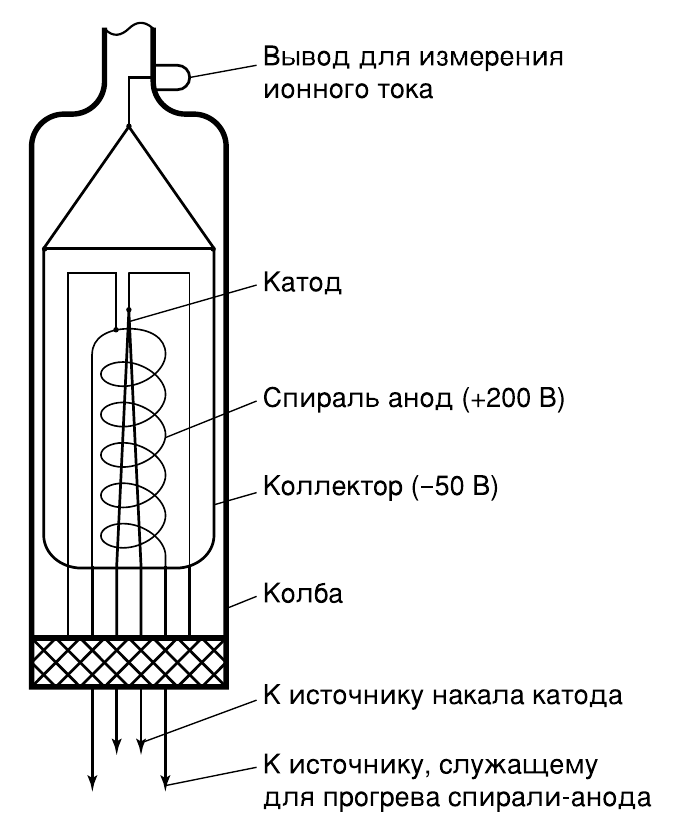
\includegraphics[width=0.5\textwidth]{ionizacionni_monometr}}
        \caption{Схема ионизационного манометра.}
        \label{ris:ionizacionni_monometr}
    \end{figure}

    \newpage

    \paragraph{Диффузионный насос:}
    Откачивающее действие диффузионногонасоса основано на диффузии (внедрении) молекул разреженного воздуха в струю паров масла. Попавшие в струю молекулы газа увлекаются ею и уже не возвращаются назад. Устройство одной ступени масляного диффузионного насоса схематически показано на (Рис. \ref{ris:diffuzionni_nasos}) (в лабораторной установке используется несколько откачивающих ступеней). Масло, налитое в сосуд А, подогревается электрической печкой. Пары масла поднимаются по трубе Б и вырываются из сопла В. Струя паров увлекает молекулы газа,которые поступают из откачиваемого сосуда через трубку ВВ. Дальше смесь попадает в вертикальную трубу Г. Здесь масло осаждаетсяна стенках трубы и маслосборников и стекает вниз, а оставшийся газчерез трубу ФВ откачивается форвакуумным насосом. Диффузионный насос работает наиболее эффективно при давлении, когда длинасвободного пробега молекул воздуха примерно равна ширине кольцевого зазора между соплом В и стенками трубы ВВ. В этом случае пары масла увлекают молекулы воздуха из всего сечения зазора. Давление насыщенных паров масла при рабочей температуре, создаваемой обогревателем сосуда А, много больше $5\cdot10^{-2}$ торр. Именно поэтому пары масла создают плотную струю, которая и увлекаетс собой молекулы газа. Если диффузионный насос включить при давлении, сравнимом с давлением насыщенного пара масла, то последнее никакой струи не создаст и масло будет просто окисляться и угорать.

    Диффузионный насос, используемый в нашей установке, имеет две ступени и соответственно два сопла (Рис. \ref{ris:nasos_irl}). Одно сопло вертикальное (первая ступень), второе сопло горизонтальное (вторая ступень). За второй ступенью имеется еще одна печь, но пар из этой печи поступает не в сопло, а по тонкой трубке подводится ближе к печке первой ступени. Эта печь осуществляет фракционирование масла. Легколетучие фракции масла, испаряясь, поступают в первую ступень, обогащая ее легколетучей фракцией масла. По этой причине плотность струи первой ступени выше и эта ступень начинает откачивать при более высоком давлении в форвакуумной части установки. Вторая ступень обогощается малолетучими фракциями. Плотность струи второй ступени меньше, но меньше и давление насыщенных паров масла в этой ступени. Соответственно в откачиваемый объем поступает меньше паров масла и его удается откачать до более высокого вакуума, чем если бы мы работали только с одной ступенью.


    \begin{figure}[h]
    \centering
    \begin{minipage}{0.35\textwidth}
        \centering
        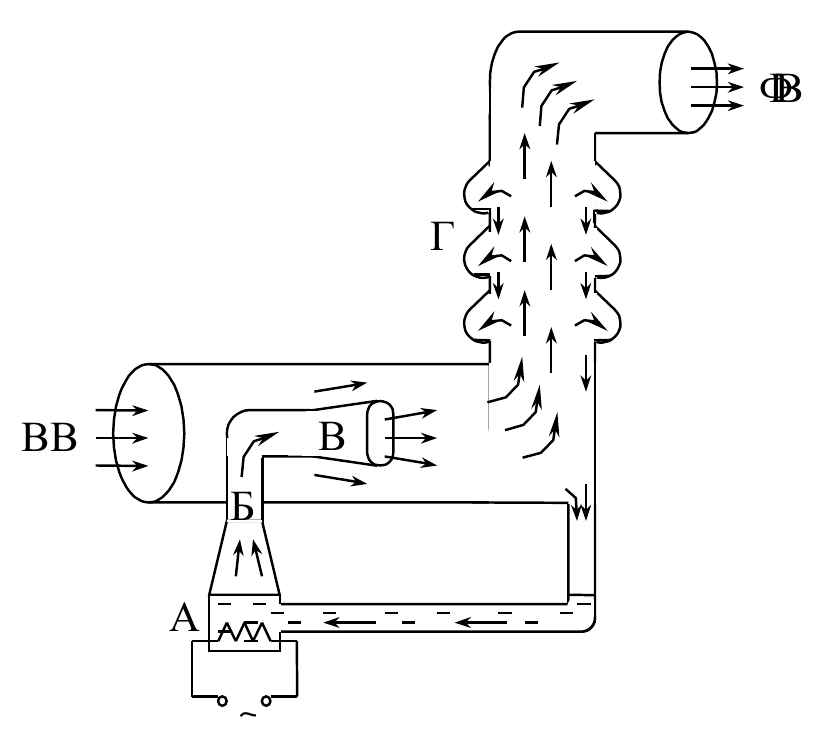
\includegraphics[width=1\textwidth]{diffuzionni_nasos}
        \caption{Схема одной ступени диффузионного насоса.}
        \label{ris:diffuzionni_nasos}
    \end{minipage}\hfill
    \begin{minipage}{0.65\textwidth}
        \centering
        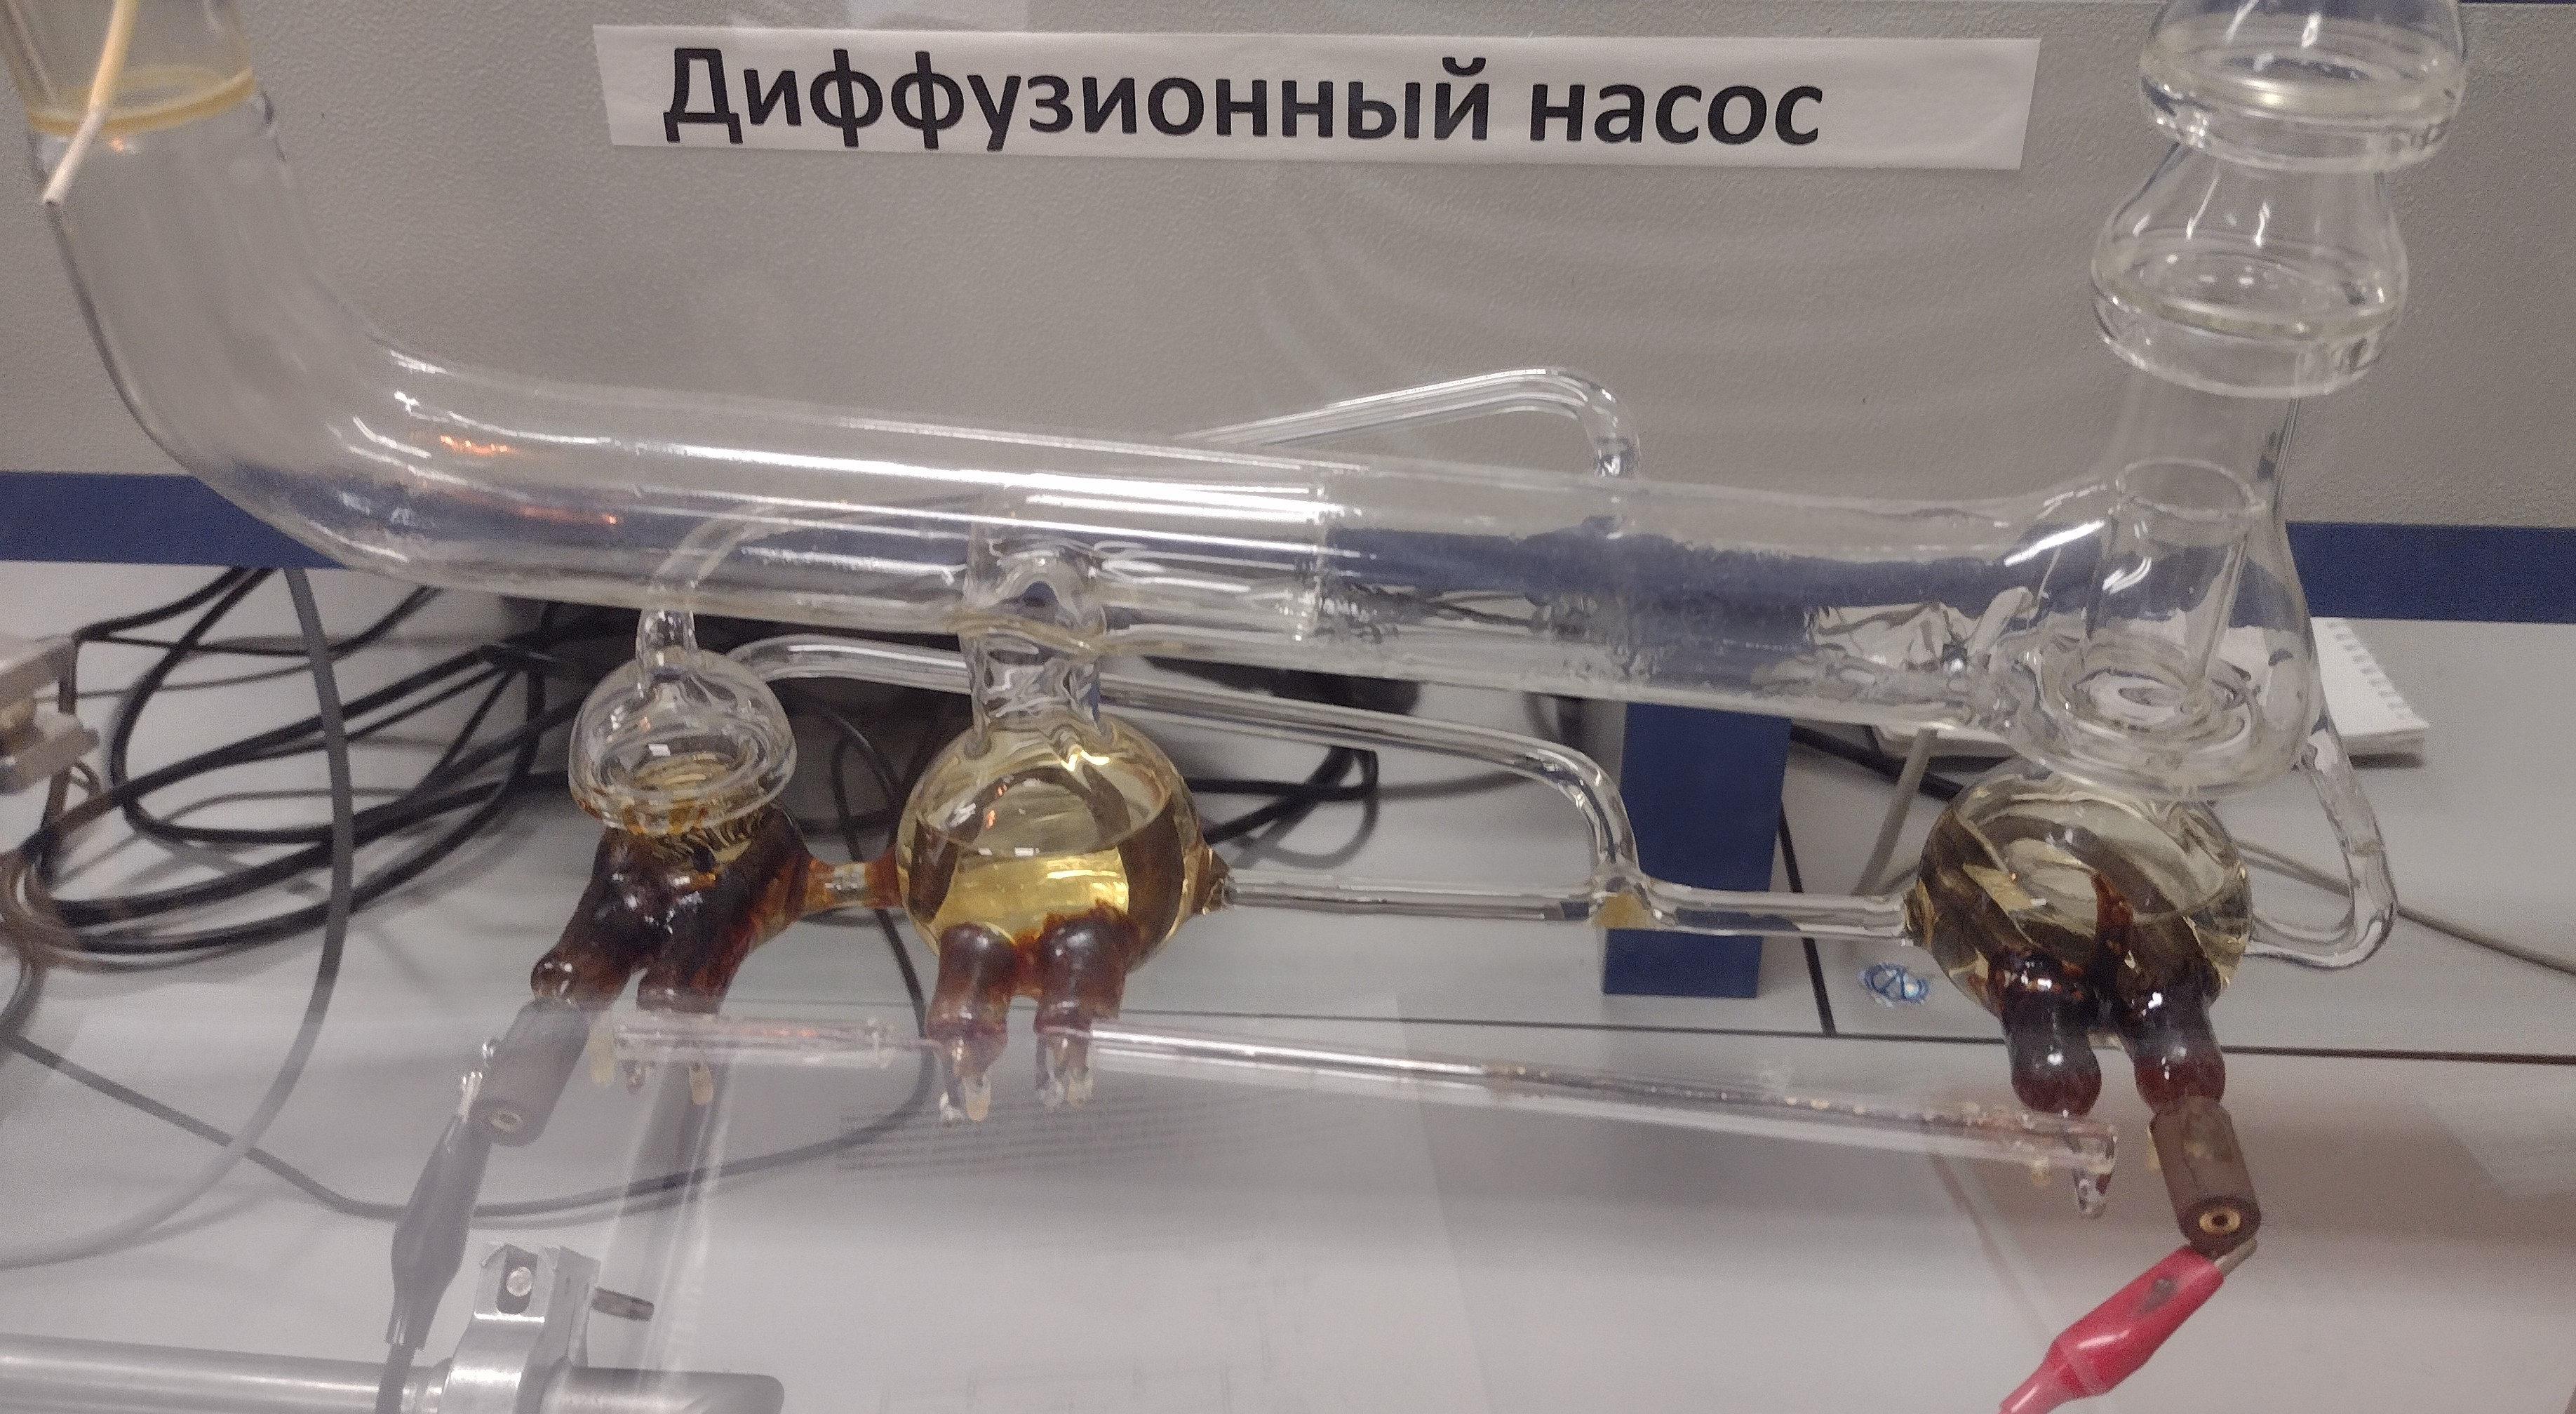
\includegraphics[width=0.9\textwidth]{nasos_irl}
        \caption{Диффузионный насос используемый в нашей работе.}
        \label{ris:nasos_irl}
    \end{minipage}
    \end{figure}


    \section{Теоретическая часть}

    \paragraph{Процесс откачки: }
    Производительность насоса определяется скоростью откачки $W$ (л/с): W — это объем газа, удаляемого из сосуда при данном давлении за единицу времени. Скорость откачки форвакуумного насоса равна емкости воздухозаборной камеры, умноженной на число оборотов в секунду.

    Обозначим через $Q_д$ количество газа, десорбирующегося с поверхности откачиваемого объема в единицу времеи, через $Q_и$ -- количество газа, проникающего в единицу времени в этот объем извне -- через течи. Будем считать, что насос обладает скоростью откачки $W$ и в то же время сам является источником газа; пусть $Q_н$ — поток газа, поступающего из насоса назад в откачиваемую систему. $Q=Q_д + Q_и + Q_н$ измеряем в единицах (моль/с). Получаем формулу
    \begin{equation*}
        -\frac{VdP}{RT}=\left(\frac{PW}{RT} - Q\right)dt
    \end{equation*}
    При предельном давлении $dP=0$ и поэтому получаем
    \begin{equation*}
        Q=\frac{P_{пр}W}{RT}
    \end{equation*}
    Подставляя получаем
    \begin{equation*}
        -VdP=W(P-P_{пр})dt
    \end{equation*}
    Интегрируем полученное ур-е и получаем
    \begin{equation}
        P-P_{пр}=(P_0 - P_{пр})\exp\left(-\frac{W}{V}t\right)
    \end{equation}
    Пренебрегая $P_{пр}$ относитеьно $P_0$
    \begin{equation}
        P=P_0\exp\left(-\frac{W}{V}t\right)
    \end{equation}
    Как видим, величина $\tau=V/W$ показывает характерное время откачки системы.

    Теперь попробуем понять чем обусловлена скорость откачки. Очевидно, скорость $W$ зависит от скорости откачки насоса $W_н$, но она так же зависит от трубопровода соединяюшего насос к откачиваемой части, т.к. если трубопровод не сможет обеспечить достаточное количество газа к входу насоса то, производительность упадет.

    \begin{figure}[h]
        \center{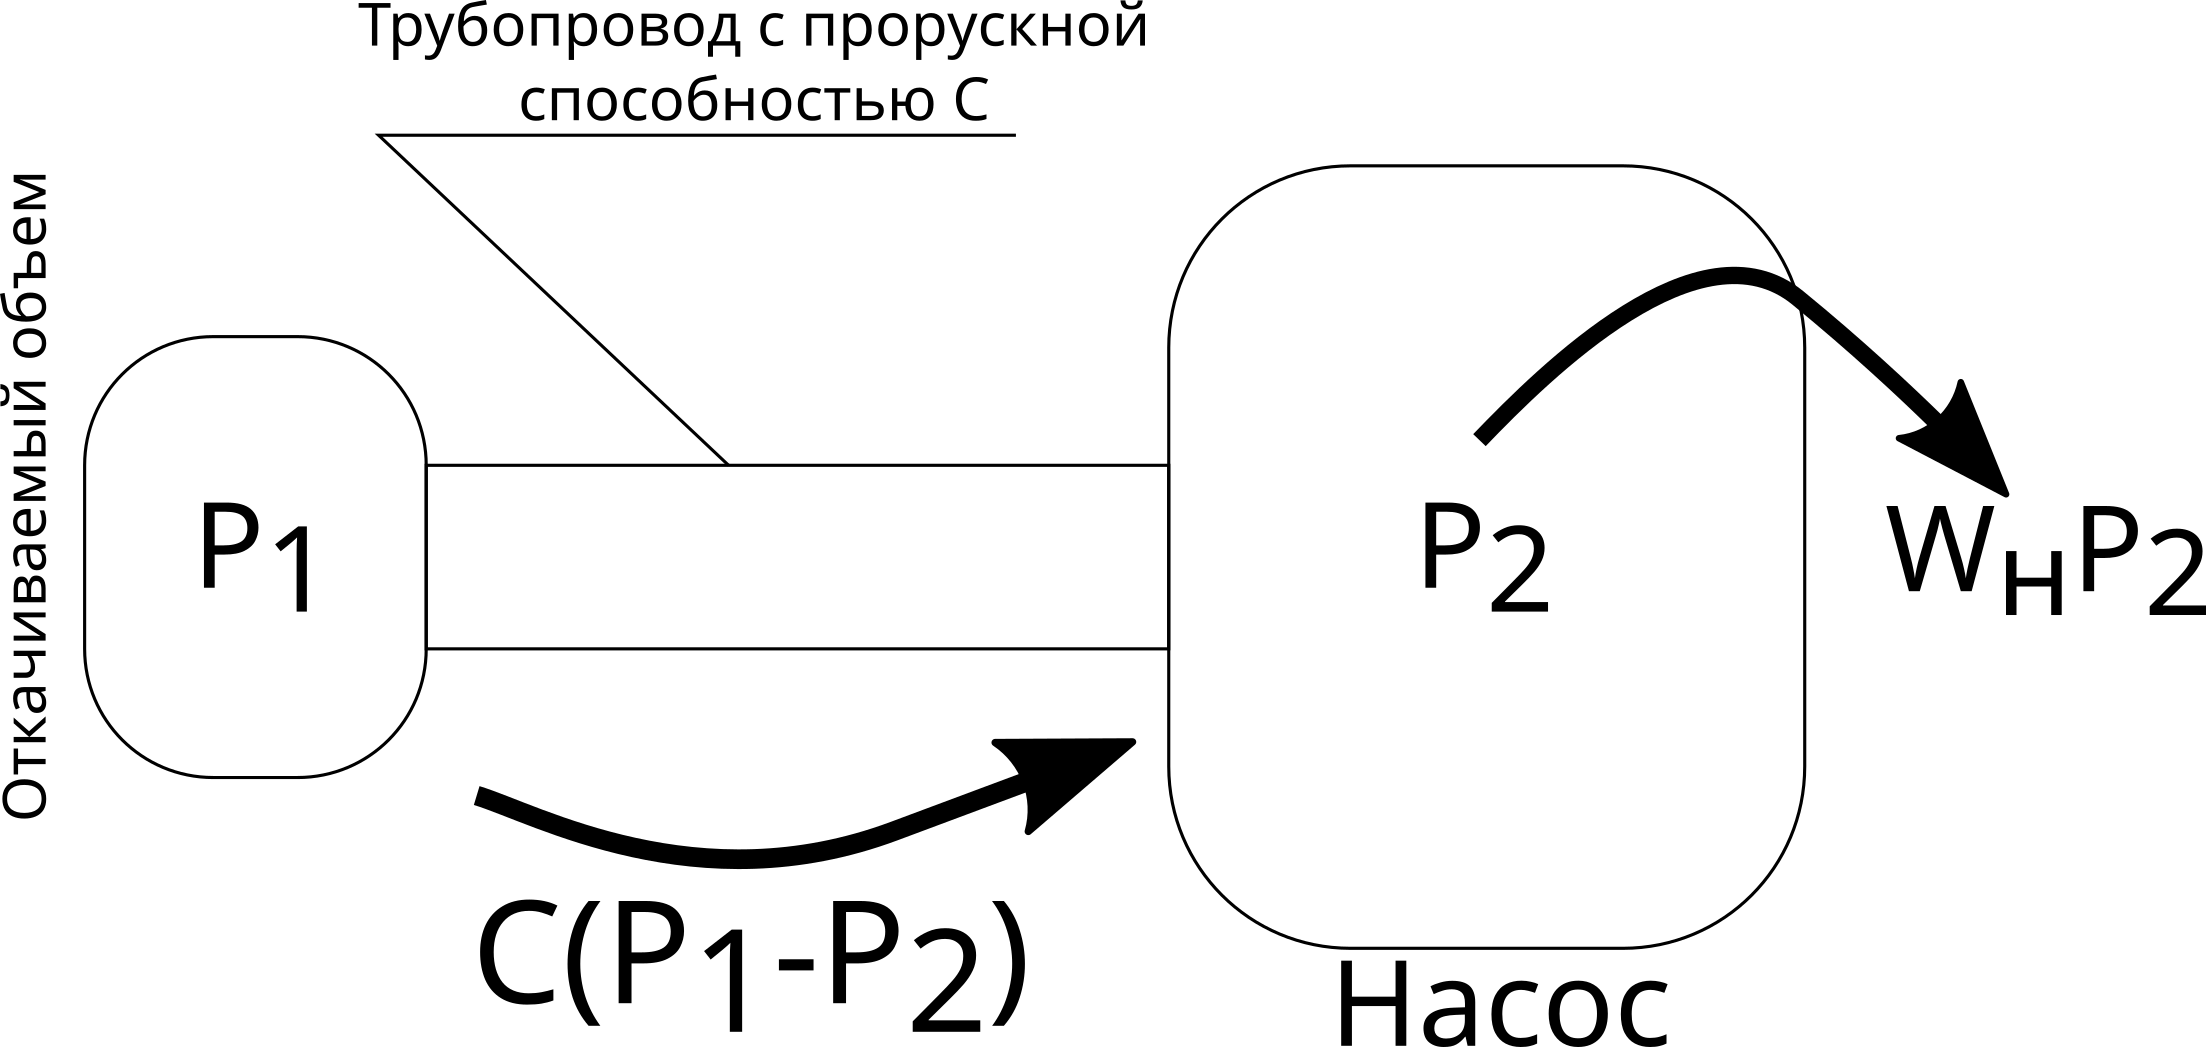
\includegraphics[width=0.7\textwidth]{nasos_sketch}}
        \caption{Схема насоса с трубопроводом.}
        \label{ris:nasos_sketch}
    \end{figure}
    Попробуем описать систему математически. Пусть у нас есть насос со скоростью откачки $W_н$ и трубопровод с пропускной способностью $C$. Давление в откачиваемом объеме -- $P_1$. Исследовав схему \ref{ris:nasos_sketch} получаем

    \begin{equation*}
        C(P_1 - P_2)=W_нP_2 \Rightarrow P_2=\frac{CP_1}{C+W_н} \Rightarrow WP_1=W_нP_2=\frac{CW_н}{C+W_н}P_1
    \end{equation*}
    Как видим, для результирующей скорости $W$ верно соотношение

    \begin{equation*}
        \frac{1}{W} = \frac{1}{W_н} + \frac{1}{C}
    \end{equation*}
    Обобщая это выражение для последовательно соединенных труб получаем

    \begin{equation}
        \frac{1}{W} = \frac{1}{W_н} + \frac{1}{C_1} + \frac{1}{C_2} + ...
        \label{resulting_speed}
    \end{equation}
    Заметим только что данные формулировки верны при молекулярном режиме течения, когда вязкое трение не имеет большого вклада в движение газа.

    \paragraph{Течение газа через трубу:} Для количества газa, протекающего через трубу в условиях высокого вакуума или, как говорят, в кнудсеновском режиме, справедлива формула

    \begin{equation}
        \frac{d(PV)}{dt} = \frac{4}{3}r^3 \sqrt{\frac{2\pi RT}{\mu}} \frac{P_2 - P_1}{L}
        \label{prop_spos_truba}
    \end{equation}
    где $r$ и $L$ соответственно радиус и длина трубы. Если пренебречь давлением $P_1$ у конца, обращенного к насосу, получаем формулу для пропускной способности трубы
    \begin{equation}
    C_{тр} = \frac{dV}{dt} = \frac{4}{3}\frac{r^3}{L}\sqrt{\frac{2\pi RT}{\mu}}
    \end{equation}
    Для пропускной способности отверстия (например в кранах) имеем формулу

    \begin{equation}
    C_{отв}=S\frac{\bar v}{4}
    \end{equation}

\end{document}
